\chapter{CSO流塑造拓扑：认知结构迁移的长期结构沉降}

\begin{chapteroverviewbox}
在前两章中，我们已经分别建立了智能系统的两个基本结构对象：一方面，认知内容及其关系构成认知结构图 $\mathcal{G}_{C}$；另一方面，承担感知、推理、控制、记忆、规划、行动等作用的功能关系构成功能拓扑 $\mathcal{G}_{F}$。二者通过随时间变化的承载映射 $\mu_t$ 联系起来。由此，一个尚未回答的根本问题自然出现：\textbf{功能拓扑为什么会形成现在的样子？为什么某些功能之间存在稳定直接连接，而另一些认知过程必须经过漫长、昂贵的中间协调？}

本章给出的回答是：\textbf{功能拓扑不是与认知活动相互独立的静态容器，而是长期认知结构流动历史的结构沉降。}当某类 Agent-CSO 长期、稳定、重复地在特定功能之间迁移，并且这种迁移具有持续任务价值时，系统具有把原本需要临时协调的动态关系固化为稳定功能耦合的动力学理由。因此：
\[
\boxed{
RepeatedCSOMigration
\longrightarrow
StableFunctionalCoupling
\longrightarrow
FunctionalTopology
}
\]
这一过程称为\textbf{拓扑沉降（Topological Sedimentation）}。

需要特别强调，本章并不把``复杂度''视为一种能够像能量一样流动的本体。早期讨论中的``复杂度迁移''在这里被重新解释为：具有具体语义与功能关系的 Agent-CSO 改变自身的表示方式、时间尺度、功能位置和承载位置，而其中长期稳定的功能迁移会进一步改变承载这些结构的功能拓扑。因此，拓扑学习并不是与 CSO 迁移平行的第五种迁移，而是\textbf{长期功能迁移在更慢时间尺度上的结构性积分结果}。

本章只讨论``CSO流如何塑造拓扑''，至于什么时候已有拓扑已经无法有效承载新的 CSO 流、什么时候应该真正触发拓扑重构，以及如何防止拓扑因短时噪声而频繁改变，将在下一章的``智能结构相变与发育''中进一步处理。
\end{chapteroverviewbox}

\begin{figure}[htbp]
\centering
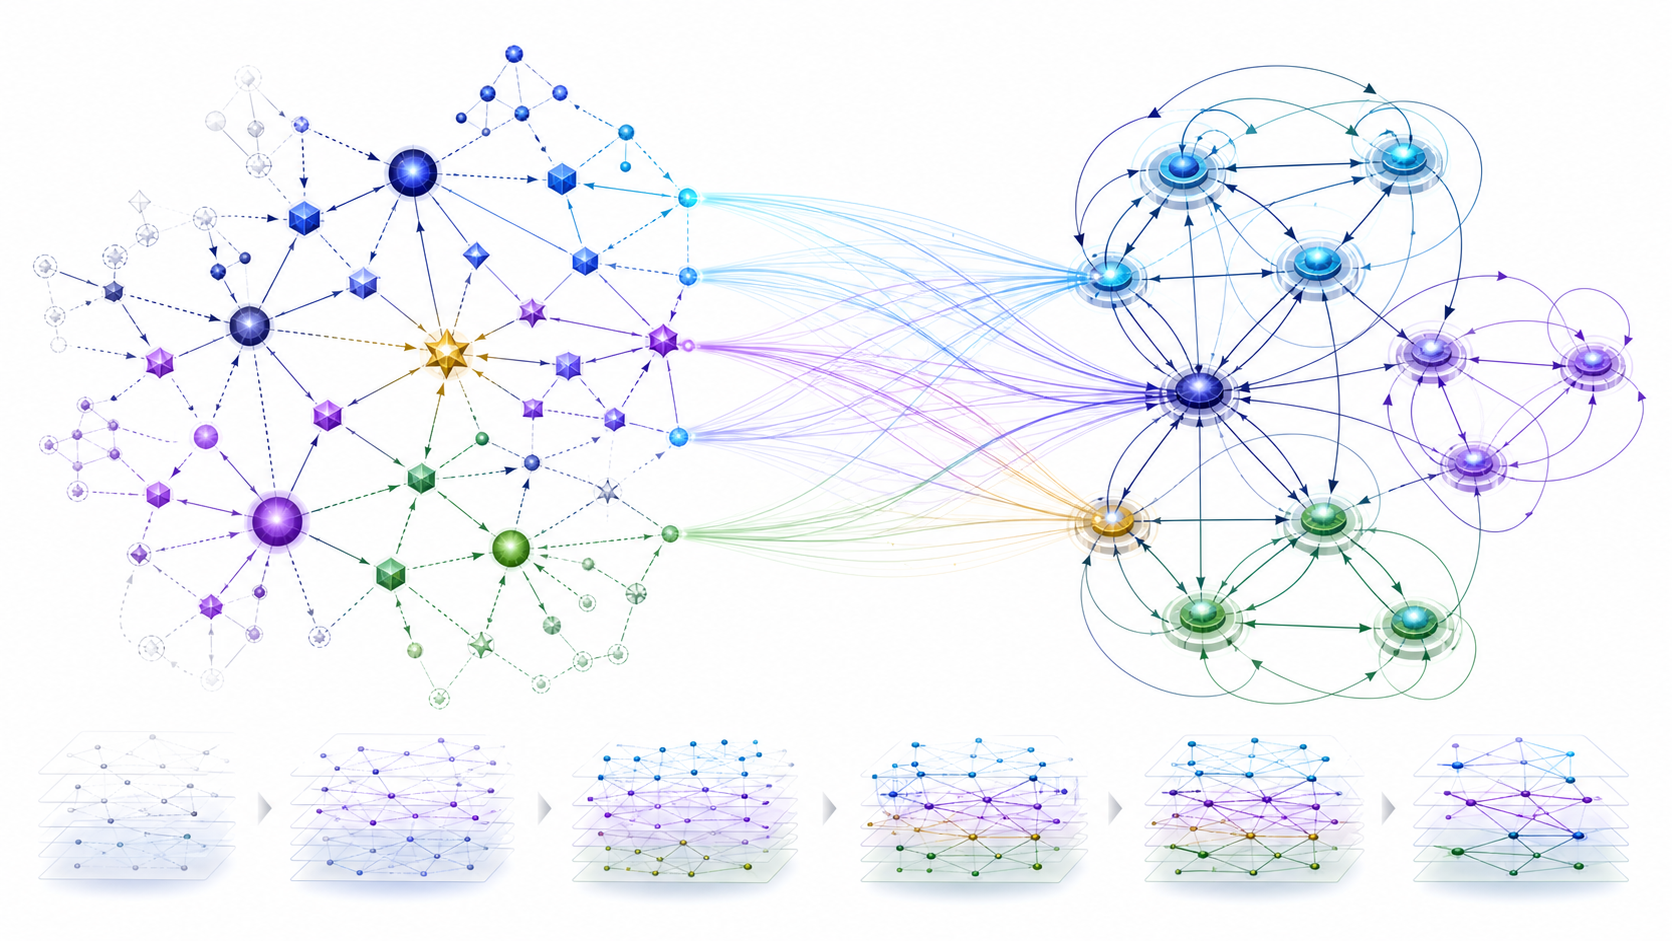
\includegraphics[width=.9\textwidth,height=.38\textheight,keepaspectratio]{images/cognitive-structure-functional-topology.png}
\caption{长期 CSO 流对功能拓扑的沉降作用}
\end{figure}
\section{从动态认知过程到稳定功能结构}

当我们观察一个刚刚接触陌生任务的智能体时，会发现大量处理过程必须通过显式认知协调完成。一个新的问题首先进入工作记忆 $h(t)$，系统需要调用不同记忆、工具、规划和预测功能，建立临时关系，再经过多轮反馈才能完成任务。此时，认知活动具有明显的``在线组装''特征：某个 Agent-CSO 并没有一个已经确定的局部处理闭环，而是在多个功能之间不断迁移。

设一个认知结构对象 $C$ 在智能体 $A$ 中的具体承载状态为
\[
X_C^A(t)
=
\left(
C,
R_C(t),
F_C(t),
\tau_C(t),
B_C(t),
S_C(t)
\right),
\]
其中 $R_C$ 表示当前表示形式，$F_C$ 表示承担该结构处理职责的功能位置，$\tau_C$ 表示其有效时间尺度，$B_C$ 表示内部或外部承载边界，$S_C$ 则表示激活、潜伏、预测、回忆等运行状态。如果我们暂时只观察功能维度，那么某次认知活动可以表示为
\[
F_C(t_0)=F_i,
\qquad
F_C(t_1)=F_j.
\]
这意味着同一 CSO 或其连续变换后的结构，从一个功能区域迁移到了另一个功能区域。

单次迁移本身并不意味着系统应该改变拓扑。智能体面对开放世界时必然会出现大量偶然的跨功能协调。例如一个罕见事故可能临时要求视觉系统、长期记忆、伦理判断、规划器和外部工具共同参与，但这种关系可能在整个生命周期只出现一次。如果系统因为任何一次临时协同都建立永久直接连接，那么拓扑会迅速膨胀，并最终失去结构性。因此我们首先必须区分：
\[
\boxed{
TransientInteraction
\neq
StructuralRelation
}
\]

真正能够形成拓扑的不是``发生过交互''，而是具有持续统计结构的交互。设功能 $F_i$ 与 $F_j$ 之间关于某类 CSO 的迁移事件序列为
\[
\mathcal{E}_{ij}^{C}
=
\left\{
e_1,e_2,\ldots,e_n
\right\}.
\]
我们可以为这些迁移定义持续性、重复性、收益性和闭环稳定性：
\[
P_{ij}^{C}
=
\operatorname{Persistence}
\left(
\mathcal{E}_{ij}^{C}
\right),
\]
\[
R_{ij}^{C}
=
\operatorname{Repetition}
\left(
\mathcal{E}_{ij}^{C}
\right),
\]
\[
U_{ij}^{C}
=
\operatorname{Utility}
\left(
\mathcal{E}_{ij}^{C}
\right),
\]
\[
L_{ij}^{C}
=
\operatorname{ClosureStability}
\left(
\mathcal{E}_{ij}^{C}
\right).
\]
只有当这些变量在足够长时间尺度上保持稳定时，动态关系才有理由逐渐沉降为结构关系。

我们由此得到本章的第一个基本判断：
\begin{proposition*}
功能拓扑不是认知活动发生之前完全给定的结构，
而可以是长期认知活动历史的压缩表示。
\end{proposition*}

这个判断与传统软件工程中的静态模块划分有明显不同。在传统软件中，架构师先规定模块 A、模块 B 和它们的接口，然后运行数据沿着预设接口流动；而在发育型智能系统中，我们考虑另一种可能性：系统首先经历大量动态 CSO 流，随后从这些长期流动关系中逐渐发现哪些功能之间值得形成稳定路径。因此功能拓扑可以被理解成：
\[
\boxed{
FunctionalTopology
=
SlowMemoryOfRepeatedFunctionalRelations
}
\]

这也解释了为什么我们此前将模块定义为
\[
Module
=
StableTopologicalCondensate.
\]
一个模块不是理论的第一性存在，它可以是大量长期反复出现的 CSO 处理关系逐渐闭合、稳定和局部化以后形成的拓扑凝聚体。换言之，智能系统中的结构并非仅仅``被设计出来''，还可能``被使用历史塑造出来''。

这里可以借鉴适应网络（adaptive network）、神经结构可塑性、编译优化和组织惯例形成等外部理论，但我们必须保持区分。Hebbian 学习研究的是活动相关性如何改变神经连接；编译器研究的是重复计算如何被优化成更直接的执行路径；组织理论研究的是重复协作怎样逐渐形成固定流程。它们都提供了``重复动态关系可以沉降为稳定结构''的外部参照，但本章的对象更加抽象：我们研究的是\textbf{跨实现、跨载体的认知结构流如何改变功能拓扑}，因此并不要求最终沉降一定表现为神经突触改变，也不要求表现为某段固定程序代码。


\section{CSO流的形式化：从承载迁移到功能通量}

为了讨论``流塑造拓扑''，我们首先需要明确这里的``流''究竟是什么。它不是抽象信息量，更不是某种实体化的复杂度，而是 Agent-CSO 在功能拓扑上的连续承载变化。假设系统具有功能节点集合
\[
V_F
=
\left\{
F_1,F_2,\ldots,F_m
\right\},
\]
认知结构对象集合
\[
V_C
=
\left\{
C_1,C_2,\ldots,C_n
\right\}.
\]
对每一个 Agent-CSO，我们可以定义一个动态承载向量
\[
\boldsymbol{\mu}_{C}(t)
=
\left[
\mu_{C1}(t),
\mu_{C2}(t),
\ldots,
\mu_{Cm}(t)
\right],
\]
其中
\[
\mu_{Ci}(t)\in[0,1]
\]
表示功能 $F_i$ 在时间 $t$ 对认知结构 $C$ 的有效承载程度，并满足近似归一化条件
\[
\sum_{i=1}^{m}
\mu_{Ci}(t)
\leq 1.
\]
这里使用``$\leq 1$''而不是严格等于 $1$，是因为部分结构可能处于外部承载、休眠、尚未被任何内部功能显式激活的状态。

于是，CSO 从功能 $F_i$ 向 $F_j$ 的迁移可以通过承载权重变化定义。最简单地，可以令
\[
J_{ij}^{C}(t)
=
\Phi_{ij}
\left(
\mu_{Ci}(t),
\mu_{Cj}(t),
\dot{\mu}_{Ci}(t),
\dot{\mu}_{Cj}(t)
\right),
\]
其中 $J_{ij}^{C}(t)$ 表示认知结构 $C$ 在功能边 $i\rightarrow j$ 上的有效功能通量。对于离散事件系统，则可以定义
\[
J_{ij}^{C}[k]
=
\begin{cases}
1,&
C\text{ 在第 }k\text{ 次事件中由 }F_i
\text{ 转入 }F_j,\\
0,&
\text{otherwise}.
\end{cases}
\]
生命周期尺度上的平均功能流可以写为
\[
\overline{J}_{ij}^{C}(T)
=
\frac{1}{T}
\int_{t-T}^{t}
J_{ij}^{C}(s)\,ds.
\]

然而，仅仅计算流量仍然不足。假设一个错误架构导致同一个 CSO 在两个模块之间不断来回传递，那么 $J_{ij}$ 很大，但我们显然不应该因为这种无效振荡而强化连接。因此真正影响拓扑学习的应该是\textbf{价值加权的有效 CSO 流}。我们可以定义
\[
\widetilde{J}_{ij}^{C}(t)
=
J_{ij}^{C}(t)
\cdot
Q_{ij}^{C}(t),
\]
其中
\[
Q_{ij}^{C}(t)
=
U_{ij}^{C}(t)
-
\lambda_r R_{ij}^{\mathrm{res}}(t)
-
\lambda_c C_{ij}^{\mathrm{coord}}(t)
-
\lambda_s S_{ij}^{\mathrm{risk}}(t).
\]
这里 $U$ 表示任务收益，$R^{\mathrm{res}}$ 表示迁移后仍残留的预测或控制残差，$C^{\mathrm{coord}}$ 表示跨功能协调成本，$S^{\mathrm{risk}}$ 表示安全与稳定性代价。于是拓扑真正应该``记住''的，不是单纯发生频繁的流，而是：
\[
\boxed{
Persistent
+
Useful
+
Stable
+
LowResidual
\quad
CSOFlow.
}
\]

进一步，如果我们不再区分具体 CSO，而考虑某一类语义结构集合 $\mathcal{C}_{\alpha}$，则可以得到功能边上的总有效通量：
\[
\mathcal{J}_{ij}^{(\alpha)}(t)
=
\sum_{C\in\mathcal{C}_{\alpha}}
\widetilde{J}_{ij}^{C}(t),
\]
以及全局功能通量矩阵
\[
\mathbf{J}_{F}(t)
=
\left[
\mathcal{J}_{ij}(t)
\right]_{m\times m}.
\]
这一矩阵并不是普通网络流量监控指标。它编码的是：\textbf{哪些功能之间正在反复承担同类认知结构的传递、变换和闭环协调。}

我们由此可以重新解释此前的``复杂度流''。在早期理论中，我们曾试图用
\[
\rho(f,\omega,t)
\]
描述复杂度在功能位置 $f$ 与频率 $\omega$ 上的分布，并引入连续性方程：
\[
\frac{\partial\rho}{\partial t}
+
\nabla\cdot\mathbf{J}
=
S-D.
\]
这一形式仍然具有价值，但本体解释应改写。更严格地，我们应令
\[
\rho_{CSO}(f,\omega,t)
\]
表示一定时间窗口内活跃或稳定 Agent-CSO 在功能—时间尺度空间中的分布，而
\[
\mathbf{J}_{CSO}(f,\omega,t)
\]
表示这些结构在该空间中的迁移通量。于是：
\[
\frac{\partial\rho_{CSO}}{\partial t}
+
\nabla_{f,\omega}\cdot
\mathbf{J}_{CSO}
=
S_{CSO}-D_{CSO},
\]
其中 $S_{CSO}$ 表示新结构形成，$D_{CSO}$ 则表示遗忘、合并、抽象或失去独立表达等过程。

因此，本章所说的 CSO 流可以在三个层次理解：微观层是单一 Agent-CSO 的功能承载变化；中观层是某一语义类结构在功能图上的统计迁移；宏观层则是整个智能体生命周期中的功能—时间尺度结构流场。后面所谓``拓扑沉降''，实际上发生在第三种视角的慢时间尺度上。


\section{从重复迁移到稳定耦合：拓扑沉降的基本机制}

现在我们可以正式回答本章的核心问题：动态 CSO 流如何变成功能拓扑？

设现有功能拓扑为
\[
\mathcal{G}_F(t)
=
\left(
V_F,
E_F(t),
W_F(t)
\right),
\]
其中 $W_F(t)=\{w_{ij}(t)\}$ 表示功能节点之间的有效耦合强度。这里的 $w_{ij}$ 不一定对应一条真实神经突触或一条固定软件函数调用，它表示的是更加抽象的\textbf{稳定功能可达性与因果耦合能力}。一个较大的 $w_{ij}$ 意味着，$F_i$ 与 $F_j$ 之间已经存在低成本、高可靠、重复可利用的处理关系。

为了描述拓扑沉降，我们引入比认知运行快环慢得多的拓扑时间常数
\[
\tau_T.
\]
若认知活动的典型时间尺度为 $\tau_C$，则应满足
\[
\boxed{
\tau_T
\gg
\tau_C.
}
\]
在 AgentOS 的整体多尺度框架下，更完整地可以写成：
\[
\tau_h
\ll
\tau_E
\ll
\tau_\Theta
\lesssim
\tau_F
\ll
\tau_T,
\]
其中 $\tau_F$ 表示显著功能职责迁移的时间尺度，而 $\tau_T$ 表示真正稳定改变功能耦合关系所需的时间尺度。

一种最小化的边权演化模型可以写成
\[
\tau_T
\dot w_{ij}
=
\alpha
\left\langle
\mathcal{J}_{ij}^{+}
\right\rangle_T
-
\beta
\left\langle
C_{ij}^{\mathrm{coord}}
\right\rangle_T
-
\gamma
\left\langle
R_{ij}^{\mathrm{res}}
\right\rangle_T
-
\delta
w_{ij},
\]
其中
\[
\mathcal{J}_{ij}^{+}
=
\max
\left(
0,
\mathcal{J}_{ij}
\right)
\]
代表能够产生正向任务价值的有效结构流，$\langle\cdot\rangle_T$ 表示在拓扑学习时间窗口上的长期平均。

这个方程表达了一个很简单但非常重要的原则：当大量有价值 CSO 长期稳定地在 $F_i$ 和 $F_j$ 之间迁移，而两者之间现有协调成本较高时，系统有动力增加直接耦合；反之，如果一条功能连接长期几乎没有产生有价值的结构流，或者不断引入残差与冲突，它就应该逐渐衰减。

于是拓扑沉降可以概括为：
\[
\resizebox{.96\linewidth}{!}{$\displaystyle
\boxed{
DynamicCoordination
\rightarrow
RepeatedCoordination
\rightarrow
PredictableCoordination
\rightarrow
DirectFunctionalCoupling.
}
$}
\]

这里存在一个关键认识：\textbf{学习不一定表现为``系统知道更多''，也可能表现为``系统以后不必再为同样的问题进行这么多全局协调''。}例如一个新任务最初可能需要：
\[
h
\rightarrow
Planning
\rightarrow
Memory
\rightarrow
Tool
\rightarrow
h
\rightarrow
Action.
\]
当这一认知路径长期重复后，它可能逐渐形成更局部的技能结构：
\[
Perception
\rightarrow
CompiledSkill
\rightarrow
Action,
\]
而原本需要显式经过 $h$ 的大量关系被沉降进新的直接功能闭环。从外部看，智能体似乎``思考得更少''；但从结构上看，它并不是知道得更少，而是：
\[
\boxed{
ThinkingLess
\neq
KnowingLess.
}
\]
更准确的描述是：
\begin{statementbox}
CognitiveStructureChangedCarrier.
\end{statementbox}

这与人类技能自动化有明显相似性。初学驾驶时，大量动作必须进入显式工作记忆；熟练之后，很多感知—动作关系转移到快速、局部和程序化闭环。类似现象也存在于软件工程：高频函数调用会被缓存、内联、编译、建立索引；组织中反复出现的协作关系会形成岗位和制度。但本理论试图把这些现象统一到一个更抽象的形式：
\[
\boxed{
RepeatedUsefulStructureFlow
\rightarrow
StableCarrierRelation.
}
\]

因此，我们可以把拓扑理解为``过去认知活动的压缩结果''。它不是传统意义上的 episodic memory，也不是 $\Theta$ 中某个纯粹世界知识结构，而是一种更深的\textbf{系统组织记忆}：系统通过自己的连接方式记住``哪些功能过去长期值得直接合作''。


\section{功能拓扑作为CSO流的慢积分：拓扑记忆模型}

如果拓扑真的是长期 CSO 流的历史沉降，那么一个自然的数学表达是：拓扑应当近似为历史有效功能流的低通积分。设功能通量矩阵为 $\mathbf{J}_F(t)$，则拓扑可以写成：
\[
\boxed{
\mathbf{W}_F(t)
=
\mathcal{H}_{T}
\left[
\mathbf{J}_F(s)
\right]_{s\leq t},
}
\]
其中 $\mathcal{H}_{T}$ 是一个慢时间尺度历史算子。在线性近似下，可以表达成指数记忆核：
\[
w_{ij}(t)
=
\int_{-\infty}^{t}
K_T(t-s)
\,
\widetilde{J}_{ij}(s)
\,ds,
\]
其中
\[
K_T(\Delta t)
=
\frac{1}{\tau_T}
e^{-\Delta t/\tau_T},
\qquad
\Delta t\geq0.
\]
于是：
\[
\boxed{
FunctionalTopology
\approx
SlowIntegralOfEffectiveCSOFlow.
}
\]

这个公式的重要之处不在于我们一定要采用指数核，而在于它揭示了一个更一般的时间尺度结构：瞬时 CSO 流是快变量，功能拓扑是对这些快变量长期统计结构进行积分后形成的慢变量。它与我们此前提出的智能频谱理论完全一致：
\[
SlowStructureShapesFastActivity,
\]
而
\[
PersistentFastResidualShapesSlowStructure.
\]

只不过在本章中，``慢结构''已经从 $\Theta$、$\Psi$ 进一步推广到功能拓扑本身。

为了避免拓扑把所有过去交互无限积累起来，我们需要引入遗忘或折旧项。于是：
\[
\tau_T\dot w_{ij}
=
G_{ij}
-
\lambda_Tw_{ij},
\]
其中
\[
G_{ij}
=
G
\left(
\langle J_{ij}\rangle,
Utility,
Residual,
CoordinationCost,
Risk
\right).
\]
$\lambda_T$ 表示拓扑关系的自然折旧速度。长期不再使用的功能关系不应永久占据结构资源，否则系统会产生``拓扑老化''：大量曾经有用但现在已经失去意义的连接继续改变路由、引入维护成本和错误先验。

从这里我们可以定义一种\textbf{拓扑记忆半衰期}：
\[
T_{1/2}^{ij}
=
\frac{\ln 2}{\lambda_{ij}},
\]
不同功能边可以具有不同的稳定程度。安全关键的基础闭环可能具有极长半衰期，实验性技能通路则可以具有较短半衰期。这与 AgentOS 的慢变量保护原则一致：
\[
\boxed{
FastNoise
\nrightarrow
SlowGlobalStructure.
}
\]

更进一步，我们还可以把拓扑看成一种第二阶记忆。第一阶记忆保存的是``发生了什么''：
\[
E:
\quad
Event/TrajectoryMemory.
\]
第二阶结构记忆保存的是``世界和技能通常怎样组织''：
\[
\Theta:
\quad
GenerativeStructure.
\]
而功能拓扑则保存：
\begin{statementbox}
系统自己过去通常怎样处理这些结构最有效。
\end{statementbox}
因此它是关于\textbf{认知组织方式本身}的长期记忆。

我们可以把这三类慢化过程写成：
\[
Experience
\rightarrow
E,
\]
\[
RepeatedExperienceRelation
\rightarrow
\Theta,
\]
\[
RepeatedFunctionalCSOFlow
\rightarrow
\mathcal{G}_F.
\]
其中前两者主要改变认知内容，第三者开始改变承载认知内容的系统结构。

这使学习出现了一个非常重要的层级：
\[
\boxed{
LearningWhat
\rightarrow
LearningHow
\rightarrow
LearningHowToOrganizeLearning.
}
\]
$E$ 更多保存``经历了什么''，$\Theta$ 更多沉降``世界和技能如何运作''，而拓扑学习开始沉降``我应该由哪些功能关系来处理这些问题''。这也是为什么拓扑学习在理论上比普通参数学习更慢、更危险，但同时也可能带来更深层的发育能力。

这里与控制理论中的慢参数自适应、机器学习中的 meta-learning、编译器中的 profile-guided optimization，以及组织理论中的 routine formation 都存在可比较之处。但本理论要求这些现象共享一个更加基础的结构解释：\textbf{稳定的快过程统计结构，能够被慢变量吸收，从而改变未来快过程的可行路径。}


\section{拓扑资本：过去协调成本如何转化为未来结构优势}

如果长期 CSO 流能够沉降成稳定拓扑，那么这种沉降为什么对智能有意义？最直接的回答是：\textbf{稳定拓扑把过去反复付出的协调成本转化为未来可以重复利用的结构优势。}我们将这种累积优势称为\textbf{拓扑资本（Topological Capital）}。

考虑某一类任务 $\mathcal{T}_{\alpha}$。在拓扑形成以前，完成该任务需要经过路径
\[
\mathcal{P}_{0}
=
F_1
\rightarrow
F_2
\rightarrow
\cdots
\rightarrow
F_k,
\]
其期望认知协调成本为
\[
C_{\mathrm{coord}}
(\mathcal{P}_{0}).
\]
在长期经验以后，系统形成了一条更直接的功能路径
\[
\mathcal{P}_{1},
\]
满足
\[
C_{\mathrm{coord}}
(\mathcal{P}_{1})
<
C_{\mathrm{coord}}
(\mathcal{P}_{0}).
\]
于是，对于任务分布 $p(\mathcal{T})$，我们可以定义拓扑资本带来的期望节省：
\[
K_T
=
\mathbb{E}_{\mathcal{T}\sim p}
\left[
C_{\mathrm{coord}}^{\mathrm{baseline}}(\mathcal{T})
-
C_{\mathrm{coord}}^{\mathrm{current}}(\mathcal{T})
\right].
\]

如果还考虑运行延迟、能耗和可靠性，则可以扩展成：
\[
K_T
=
\mathbb{E}_{\mathcal{T}}
\left[
\Delta C
+
\lambda_L\Delta L
+
\lambda_E\Delta E
+
\lambda_R\Delta R
\right],
\]
其中 $\Delta C$ 表示认知协调成本下降，$\Delta L$ 表示延迟下降，$\Delta E$ 表示能耗下降，$\Delta R$ 表示可靠性提升。

这一概念帮助我们重新理解``熟练''。熟练并不只是同一模型产生更正确答案，而是：
\begin{statementbox}
过去需要临时全局协调的结构，
逐渐被固化成低成本、局部、稳定的功能通路。
\end{statementbox}
因此我们此前提出：
\[
\boxed{
Skill
=
CSOFunctionalDownMigration.
}
\]
从本章角度，更完整的表达是：
\[
\boxed{
SkillFormation
=
CSOMigration
+
LocalClosure
+
TopologicalCapitalAccumulation.
}
\]

拓扑资本具有典型的``前期投资、后期摊销''结构。假设建立一条新功能耦合需要一次性成本
\[
C_{\mathrm{build}},
\]
每次使用它能够节省
\[
\Delta c.
\]
如果预计未来使用次数为 $N$，则建立该连接的净收益近似为
\[
V_{\mathrm{edge}}
=
N\Delta c
-
C_{\mathrm{build}}
-
C_{\mathrm{maintain}}
-
C_{\mathrm{risk}}.
\]
只有当
\[
V_{\mathrm{edge}}>0
\]
时，拓扑沉降才具有长期经济性。

这解释了为什么一个智能体不应该把所有偶发处理都编译成新模块。拓扑是一种昂贵资源。它带来速度和稳定性，但也带来维护成本、僵化风险和错误固化风险。每一条新功能边实际上都是对未来任务分布的一种长期赌注：
\[
\boxed{
NewTopology
=
CommitmentToFutureRegularity.
}
\]

如果环境长期稳定，这种赌注可以产生巨大的结构资本；如果环境突然变化，过去形成的拓扑资本甚至可能变成拓扑负债。例如，一个高度专门化的技能系统在原任务上极为高效，但进入新环境以后可能因为过强的旧闭环而产生偏差。因此：
\[
\boxed{
TopologicalCapital
\neq
UnconditionalAdvantage.
}
\]

它只在未来任务统计结构与过去具有一定连续性时成立。

从这个角度看，人类专家、成熟企业和长期 Agent 都会表现出类似现象：它们不是因为每一刻都进行更多计算而强大，而是因为过去大量昂贵协调已经被沉积进结构。因此成熟智能的一项重要指标可能不是``单位时间显式推理量''越来越大，而是：
\[
\boxed{
\frac{
ExplicitGlobalCoordinationCost
}{
SuccessfulBehavior
}
\downarrow.
}
\]

这与全书后续所强调的
\[
MatureIntelligence
=
SelectiveExplicitCognition
\]
直接相连。真正成熟的系统，应该把有限工作记忆 $h$ 留给新颖、冲突、异常和真正需要跨域整合的问题，而不是让已经重复千百次的稳定关系永久占据全局认知资源。


\section{拓扑学习不是独立迁移维度：从CSO迁移到结构沉降}

在早期的复杂度迁移理论中，我们曾经尝试把智能变化拆解为多个彼此平行的方向，其中包括功能迁移、频率迁移、边界迁移以及拓扑变化。随着 CSO 本体逐渐清晰，我们需要对这一分类作出一个重要修正：\textbf{拓扑学习不应被理解成与表示、功能、时间尺度和边界迁移并列的第五种 CSO 迁移。}

对于一个具体 Agent-CSO，我们可以定义基本迁移向量：
\[
\boxed{
\mathcal{M}_{CSO}
=
\left(
M_R,
M_F,
M_\tau,
M_B
\right)
}
\]
其中
\[
M_R
\]
表示表示形式变化，例如自然语言显式步骤被压缩成结构表示；
\[
M_F
\]
表示功能承担位置变化，例如一个问题从全局规划功能迁移到局部 Skill；
\[
M_\tau
\]
表示时间尺度变化，例如活跃结构逐渐凝固为长期生成结构；
\[
M_B
\]
表示边界迁移，例如内部结构被外化为工具、文件、代码或环境状态。

而功能拓扑
\[
\mathcal{T}
\]
并不是某个单一 CSO 自身的坐标。它描述的是\textbf{承载大量 CSO 的功能系统之间的关系结构}。因此：
\[
\boxed{
\Delta\mathcal{T}
\notin
\mathcal M_{CSO}
}
\]
更合理的关系是：
\[
\boxed{
PersistentM_F
\longrightarrow
\Delta\mathcal{T}.
}
\]
即长期稳定的功能迁移最终改变功能拓扑。

这一区分非常重要，因为它把``学习''与``发育''区分开来。一个 Agent-CSO 从 $F_i$ 移动到 $F_j$：
\[
CSO@F_i
\rightarrow
CSO@F_j
\]
可以是一次普通学习或运行适应；只有当大量类似关系在长期历史中重复出现，系统才可能改变
\[
w_{ij},
\]
甚至新建功能节点、拆分原有节点或形成新的闭环。于是：
\[
\boxed{
Learning
=
ChangeOfCSORealization,
}
\]
而更深层的：
\[
\boxed{
Development
=
PersistentCSOMigration
\rightarrow
FunctionalTopologyEvolution.
}
\]

从时间尺度上看，这意味着：
\[
\tau_{\mathrm{state}}
\ll
\tau_{\mathrm{representation}}
\ll
\tau_{\mathrm{spectrum}}
\lesssim
\tau_{\mathrm{function}}
\ll
\tau_{\mathrm{topology}}.
\]
这种时间尺度分离并非数学装饰，而是系统稳定性的基础。如果拓扑与当前状态一样快速变化，那么系统会失去对自己结构的可靠估计：一个控制器刚刚学习到某功能关系，下一时刻该关系已经被重写；Memory 还没有完成对上一阶段经验的结构化，承载这些经验的功能结构又发生变化。最终整个系统会成为没有稳定参考系的共同漂移系统。

因此我们提出：
\[
\boxed{
SlowVariableProtectionPrinciple:
\qquad
FastNoise
\nrightarrow
SlowGlobalStructure.
}
\]

拓扑学习必须通过统计积累、价值验证和慢时间尺度门控实现，而不能对每一次局部残差直接响应。

这一点也与 AgentOS 第一代``固定功能拓扑''设计形成连续关系。第一代 AgentOS 并不要求系统在线修改核心结构，它首先通过 $h/E/\Theta/\Psi/\Omega$、SPC、AHC、TCE、CCM、Boundary 和 Offloading 实现高度丰富的\textbf{拓扑内适应}。只有当这些低成本调整长期无法解决结构失配时，才有必要进一步进入拓扑学习。因此本章并不是推翻固定拓扑 AgentOS，而是说明它在更长生命周期之后可能自然进入下一层发育阶段：
\[
\resizebox{.96\linewidth}{!}{$\displaystyle
\boxed{
StateAdaptation
\rightarrow
RepresentationAdaptation
\rightarrow
TimescaleMigration
\rightarrow
FunctionalMigration
\rightarrow
TopologyEvolution.
}
$}
\]

下一章我们还会进一步把这一序列扩展成``最小必要重组原则''，使系统始终优先使用较浅、较可逆、较低成本的适应机制，而把拓扑修改保留为真正的慢结构变化。


\section{拓扑反过来塑造未来CSO流：双向共同演化}

如果本章只得出
\[
CSOFlow\rightarrow Topology
\]
还不够，因为一旦拓扑形成，它就会立即改变下一轮 CSO 流。由此我们得到整个认知结构动力学中极为重要的一对关系：
\begin{statementbox}
CSOFlowShapesTopology
\end{statementbox}
和
\begin{statementbox}
TopologyShapesFutureCSOFlow.
\end{statementbox}

设一个 Agent-CSO 当前承载状态为 $\boldsymbol{\mu}_C(t)$，功能拓扑邻接矩阵为
\[
\mathbf{A}(t)
=
[a_{ij}(t)].
\]
则结构在功能图上的迁移概率可以表示为：
\[
P
\left(
F_C(t+\Delta t)=F_j
\mid
F_C(t)=F_i
\right)
=
\frac{
a_{ij}(t)
\exp
\left(
-\beta Cost_{ij}(C,t)
+\gamma Affinity_{ij}(C,t)
\right)
}{
Z_i
},
\]
其中 $Affinity$ 表示该功能通路对当前结构类型的匹配程度，$Cost$ 表示延迟、认知资源、风险和协调代价，$Z_i$ 为归一化项。

由这个关系可以看到，一旦某条边被长期强化：
\[
a_{ij}\uparrow,
\]
未来类似 CSO 就更容易沿着该路径流动。于是过去的历史形成拓扑，拓扑又成为未来认知活动的先验：
\[
\boxed{
PastInteraction
\rightarrow
PresentTopology
\rightarrow
FutureInteraction.
}
\]

这使智能系统产生真正意义上的历史依赖性。两个初始架构完全相同的 Agent，如果长期经历不同环境，其 CSO 流分布不同，就可能形成不同功能拓扑：
\[
\mathcal T_A(t)
\neq
\mathcal T_B(t).
\]
随后，即使二者面对相同的新问题，因为拓扑已经不同，它们也可能采用完全不同的认知路径。这意味着个体差异并不仅存在于 Memory 内容，还可能存在于：
\begin{statementbox}
HowTheAgentIsOrganizedToThink.
\end{statementbox}

我们可以把整个过程写成一个耦合自适应网络系统。认知状态满足：
\[
\dot{\mathbf{x}}
=
F
\left(
\mathbf{x},
\mathbf{A},
\mathbf{u},
\mathbf{w}
\right),
\]
而拓扑满足：
\[
\tau_T
\dot{\mathbf{A}}
=
G
\left(
\langle\mathbf{J}_{CSO}\rangle_T,
\langle\boldsymbol{\varepsilon}\rangle_T,
Utility,
Cost,
Risk
\right).
\]
于是：
\[
\boxed{
\mathbf{x}
\longrightarrow
\mathbf{J}_{CSO}
\longrightarrow
\mathbf{A}
\longrightarrow
\mathbf{x}'.
}
\]

这正是所谓
\[
\boxed{
DynamicsOnTopology
+
DynamicsOfTopology.
}
\]

前者研究在给定功能拓扑上智能如何运行；后者研究长期运行历史如何改变拓扑本身。二者不能被分开理解。

这一框架与适应网络（adaptive/co-evolving networks）理论存在直接形式相似性。在传统网络动力学中，节点状态通过网络传播，而节点状态反过来改变网络边；例如社会意见影响社交关系，社交关系又改变未来意见传播。在我们的理论中，传播的对象不是简单标量状态，而是具有语义、时间尺度、边界和功能角色的 Agent-CSO。因此我们所研究的是一种更加具体的认知—功能共同演化：
\[
\boxed{
CognitiveStructureDynamics
\bowtie
FunctionalTopologyDynamics.
}
\]

这也意味着拓扑最终会形成``认知吸引路径''。当某一类结构长期沿着同一组功能流动以后，系统遇到类似问题时会自然优先进入这些路径。这可以带来专家直觉，也可能形成路径依赖、刻板反应甚至错误习惯。因此，拓扑不仅是一种能力结构，也是一种偏置结构：
\[
\boxed{
Topology
=
Capability
+
Constraint.
}
\]
它让某些认知过程变得非常容易，同时让其他可能路径变得不再容易被探索。

因此成熟智能必须同时具有两种能力：第一，利用稳定拓扑获得高效率；第二，在拓扑与现实长期失配时重新打开原本被压缩的搜索空间。这正是下一章``结构失配—拓扑压力—拓扑相变''需要进一步处理的问题。


\section{拓扑沉降的判据：什么样的CSO流值得被写入结构}

如果任何重复活动都能够直接形成拓扑，系统必然会产生错误固化。因此，必须明确什么样的 CSO 流才具有成为稳定结构的资格。我们可以把这种资格概括成五个主要条件：持续性、收益性、可预测性、局部可闭合性和现实可验证性。

首先是持续性。设观察窗口为 $T$，定义边 $i\rightarrow j$ 上的持续结构流强度：
\[
P_{ij}(T)
=
\frac{1}{T}
\int_{t-T}^{t}
\mathbb{I}
\left(
J_{ij}(s)>\epsilon_J
\right)
ds.
\]
只有当
\[
P_{ij}(T)>\theta_P
\]
并持续足够时间，系统才应该认为这不是偶然交互。

第二是收益性。我们定义：
\[
U_{ij}(T)
=
\mathbb E_T
\left[
Reward
-
Cost
-
Risk
\right].
\]
只有：
\[
U_{ij}(T)>\theta_U
\]
的迁移关系才具有正向沉降价值。这里的 Reward 不应只理解成外部奖励，它也可以是预测误差下降、任务闭合率提高、延迟降低或认知负载减少。

第三是可预测性。如果相同 CSO 从 $F_i$ 出发后有时需要 $F_j$、有时需要 $F_k$、有时完全不需要下游功能，那么建立固定连接未必合理。因此需要：
\[
H
\left(
F_{next}\mid C,F_i
\right)
<
\theta_H,
\]
即下一功能位置的条件熵足够低。一个稳定拓扑边应该对应相对稳定的未来功能关系。

第四是局部可闭合性。我们此前反复提出：
\begin{statementbox}
EachScaleShouldCloseItsOwnFastLoop.
\end{statementbox}
若某类问题在 $F_i$ 与 $F_j$ 的局部组合中已经可以稳定完成，而无需反复提升到更高层：
\[
Residual_{local}
<
\epsilon,
\]
则它特别适合沉降成局部功能闭环。反之，如果完成该任务仍长期依赖广泛世界模型、价值判断或全局规划，那么过早局部化会造成危险。

第五也是最重要的一条，是现实可验证性：
\begin{statementbox}
RealityIsUltimateConstraint.
\end{statementbox}
一个内部关系即使极其稳定，如果它只是错误自证循环，也不能成为可靠拓扑。例如错误的 Self Interpretation 可能导致注意偏置，注意偏置产生选择性经验，选择性经验又不断强化原解释。内部流量可以非常高，却不代表它是真实有效结构。因此拓扑沉降必须保留外部验证项：
\[
V_{world}
=
Consistency
\left(
Prediction,
ActionOutcome,
Observation
\right).
\]
只有：
\[
V_{world}>\theta_V
\]
时，内部重复关系才有资格获得更高结构稳定性。

综合起来，我们可以定义一个拓扑沉降评分：
\[
\Sigma_{ij}
=
\alpha_P P_{ij}
+
\alpha_U U_{ij}
-
\alpha_H H_{ij}
+
\alpha_L L_{ij}
+
\alpha_V V_{ij}
-
\alpha_R Risk_{ij}.
\]
若
\[
\Sigma_{ij}
>
\theta_{\mathrm{sediment}}
\]
并持续
\[
T>T_{\min},
\]
则允许：
\[
w_{ij}\uparrow.
\]

这里仍然不意味着立即改变物理结构。在实际 AgentOS 工程中，功能拓扑强化可以有多个实现层级。例如：
\[
\begin{aligned}
&\text{RoutingPreference},\\
&\text{CachedPath},\\
&\text{DirectAPI},\\
&\text{CompiledSkill},\\
&\text{LearnedAdapter},\\
&\text{DedicatedController},\\
&\text{NewPersistentService}.
\end{aligned}
\]
这些实现的物理形式完全不同，但它们都实现同一功能效果：减少某类稳定 CSO 流所需要的动态协调长度。因此我们必须再次区分：
\[
\boxed{
FunctionalTopologyChange
\neq
PhysicalRewiringOnly.
}
\]

这也是本理论能够同时适用于神经系统、软件 Agent、机器人和组织系统的重要原因。


\section{拓扑迟滞与慢变量保护：防止结构追随噪声}

虽然真正的拓扑相变将在下一章讨论，但本章必须先处理一个直接问题：如果边权根据长期 CSO 流更新，如何避免系统在临界区域不断建立、删除、重新建立同一功能关系？

解决办法是引入\textbf{拓扑迟滞（Topological Hysteresis）}。

对于尚不存在的功能边，定义建立阈值：
\[
\theta_{\mathrm{on}},
\]
对于已经存在的功能边，定义删除阈值：
\[
\theta_{\mathrm{off}},
\]
并要求：
\[
\boxed{
\theta_{\mathrm{on}}
>
\theta_{\mathrm{off}}.
}
\]

新边只有在：
\[
\Sigma_{ij}>\theta_{\mathrm{on}}
\]
并持续足够长时间以后才建立；但已经建立的边不会因为评分短暂下降就立即删除，只有当：
\[
\Sigma_{ij}<\theta_{\mathrm{off}}
\]
并持续相当时间以后才逐渐衰减。

因此：
\[
\boxed{
FormationRequiresStrongEvidence,
DeletionRequiresPersistentDisuse.
}
\]

这种迟滞结构可以避免短期环境变化导致系统整体结构振荡。它和人类技能、组织制度以及成熟软件接口都具有相似直觉：建立一个稳定结构往往需要大量证据，但结构一旦形成，也不会因为一次失败就完全消失。

进一步，我们可以定义拓扑更新的最大速率：
\[
\left|
\dot w_{ij}
\right|
\leq
\kappa_T,
\]
以及全局拓扑变化预算：
\[
\sum_{ij}
\left|
\Delta w_{ij}
\right|
\leq
B_T.
\]
$B_T$ 可以理解成一定生命周期窗口内允许消耗的\textbf{拓扑可塑性预算}。这与后期 AgentOS 中的 Adaptation Budget 思想是一致的：慢结构并不是永远不能改变，而是它们的改变必须受预算和治理。

若未来进一步允许节点生成与删除，还可以定义：
\[
N_{\mathrm{rewrite}}
(T)
\leq
B_{\mathrm{rewrite}},
\]
避免系统长期处于持续 architecture search 状态。

这里与经典控制理论中的 gain scheduling、鲁棒性裕量和慢参数自适应，以及机器学习中的 stability--plasticity dilemma 都存在理论联系。智能系统需要同时满足：
\begin{statementbox}
PlasticEnoughToLearn
\end{statementbox}
和
\begin{statementbox}
StableEnoughToRemainItself.
\end{statementbox}
这种张力不仅存在于参数和记忆，也存在于功能拓扑。

从 AgentOS 的生命周期角度看，越慢、越接近身份与基础能力的结构，其修改阈值越高。因此可以建立：
\[
\theta_{\mathrm{on}}^{fast}
<
\theta_{\mathrm{on}}^{skill}
<
\theta_{\mathrm{on}}^{core}
<
\theta_{\mathrm{on}}^{identity}.
\]
这与
\[
\tau_h
\ll
\tau_E
\ll
\tau_\Theta
\ll
\tau_\Psi
\ll
\tau_\Omega
\]
共同构成一种统一原则：\textbf{结构越接近生命周期底层生成约束，就越必须用更长历史和更强现实证据才能改变。}

因此，拓扑学习不是自由重写自身。恰恰相反，一个成熟的拓扑学习系统应该表现出非常强的保守性：绝大多数短期变化首先由状态调节、表示改变、CCM、Boundary、Offloading 和功能迁移吸收，只有持续无法被这些较浅机制解决的结构关系，才会逐渐进入拓扑沉降。这一思想将在下一章正式发展成：
\begin{statementbox}
MinimumNecessaryReorganizationPrinciple.
\end{statementbox}


\section{本章的理论依赖、可验证预测与边界}

我们最后需要把本章放回已有科学与整个 AgentOS 理论之间，明确哪些部分属于外部理论支撑，哪些属于结构类比，哪些则是本书提出的待验证假说。

第一类外部依赖来自\textbf{适应网络与共演化网络理论}。这类理论已经广泛研究节点状态与网络结构双向影响的动力系统：
\[
\dot x_i
=
F_i(x,A),
\qquad
\dot A
=
G(A,x).
\]
本章借用了这一基本数学形式，但将节点状态替换为具有语义本体、功能位置、时间尺度和载体信息的 Agent-CSO 流。因此我们不能简单声称 CSO 理论等同于 adaptive network theory；更准确的说法是，适应网络为``Dynamics on Topology + Dynamics of Topology''提供成熟的数学工具。

第二类依赖来自\textbf{慢—快动力系统与平均理论}。拓扑被建模为对快速功能交互的长期统计积分，因此：
\[
\tau_{\mathrm{cognition}}
\ll
\tau_{\mathrm{topology}}.
\]
这与 singular perturbation、averaging 和 slow manifold 理论具有明确形式联系。未来如果需要严格证明拓扑更新不会破坏快系统稳定性，可以尝试建立：
\[
\epsilon
=
\frac{
\tau_{\mathrm{fast}}
}{
\tau_{\mathrm{slow}}
}
\ll1
\]
条件下的稳定性与收敛分析。

第三类依赖来自\textbf{结构可塑性与程序化学习}。神经科学中的结构突触可塑性、人类技能自动化、机器学习中的 policy distillation、软件系统中的 profile-guided optimization 和编译缓存，都说明重复动态过程可能形成更直接、更低成本的稳定执行结构。它们为本理论提供现象学参照，但 CSO 拓扑理论试图建立的是实现无关层面的共同抽象。

第四类依赖来自\textbf{组织学习与制度演化}。一个组织中长期重复的信息与决策路径会逐渐形成岗位、协议和制度；一旦制度形成，又反过来约束未来信息流。这与：
\[
CSOFlow
\leftrightarrow
FunctionalTopology
\]
具有高度形式相似性。因此本章理论未来可以自然扩展到多 Agent 和文明尺度，但不能因为形式同构就自动假设所有组织结构都遵循完全相同的微观机制。

在经验层面，本章至少给出六项可以被验证或证伪的预测。

其一，如果某类 CSO 长期沿相同功能路径流动，那么允许拓扑适应的系统应逐渐降低：
\[
ExplicitCoordinationCost.
\]

其二，随着技能成熟，应观察到：
\[
h\text{介入率}\downarrow,
\]
同时局部功能闭环调用比例上升。

其三，在控制任务分布保持稳定时，具有拓扑沉降机制的 Agent 应比完全固定拓扑 Agent 表现出更低长期运行成本和更短处理路径。

其四，如果突然改变任务分布，过度沉降的系统应出现可测量的路径依赖，表现为旧拓扑带来的适应滞后。

其五，使用迟滞和慢变量保护的系统，其长期功能拓扑方差应显著低于无保护结构学习系统，同时保持相近或更好的长期收益。

其六，在相同基础模型与相同初始功能架构下，给予两个 Agent 长期不同经验，应能够形成不同的有效功能拓扑，并进一步导致面对同一新问题时产生不同的认知路径。

这些预测使本章理论不只是一个解释性隐喻，而开始具有工程和实验含义。

同时，我们必须保留三个明确边界。

第一，本章没有证明任何智能系统都必须进行拓扑学习。一个固定拓扑系统仍然可以通过参数、记忆、工具和外部结构实现高度复杂的持续学习。

第二，本章没有宣称功能拓扑必须对应神经或软件的物理重新布线。功能因果关系、路由优先级、编译技能、接口固化和专用控制器，都可以构成功能拓扑变化。

第三，本章没有证明``重复使用必然产生最佳结构''。重复关系也可能是错误习惯、病理循环或环境偶然性。因此：
\[
RepeatedFlow
\]
必须经过
\[
Utility,
RealityVerification,
Risk,
Stability
\]
等多重评价，才能进入结构沉降。


\section{小结：拓扑是历史CSO流的结构化记忆}

本章完成了从``认知结构在功能拓扑上运行''到``认知结构反过来塑造功能拓扑''的理论跃迁。

我们首先把 Agent-CSO 的功能变化定义为承载迁移，并用
\[
J_{ij}^{C}
\]
描述结构在功能节点之间的有效通量。随后指出，单次迁移不构成拓扑，只有长期、重复、有价值、低残差、现实可验证的 CSO 流，才具有沉降为稳定功能耦合的资格。

因此：
\[
\boxed{
RepeatedCSOMigration
\rightarrow
StableFunctionalCoupling
\rightarrow
FunctionalTopology.
}
\]

进一步，我们把功能拓扑理解为 CSO 流的慢时间尺度积分：
\[
\boxed{
FunctionalTopology
\approx
SlowIntegralOfEffectiveCSOFlow.
}
\]
拓扑由此获得一种特殊的记忆含义：$E$ 记住``经历了什么''，$\Theta$ 记住``结构如何生成与运作''，而功能拓扑记住的是：
\begin{statementbox}
系统自己过去怎样组织认知活动最有效。
\end{statementbox}

这种长期结构沉降能够形成\textbf{拓扑资本}。过去反复支付的显式协调成本，被逐渐转化为未来能够直接复用的功能通路。因此，一个智能系统的成熟并不意味着越来越多认知都进入工作记忆，恰恰相反，它往往意味着越来越多稳定结构从显式全局认知中下沉：
\[
ExplicitCognition
\rightarrow
StableLocalClosure.
\]
于是：
\[
\boxed{
ThinkingLess
\neq
KnowingLess.
}
\]
很多时候，它意味着系统已经把过去的思考转化成了现在的结构。

本章同时完成了一项重要概念修正：拓扑学习不是 CSO 迁移的独立维度。基本 CSO 迁移仍然只有表示、功能、时间尺度和载体等方向：
\[
\mathcal M_{CSO}
=
(M_R,M_F,M_\tau,M_B),
\]
而：
\[
\boxed{
PersistentM_F
\rightarrow
\Delta\mathcal T.
}
\]
拓扑变化是长期功能迁移的结构性沉降，因此它属于比普通学习更慢的发育过程。

最终，我们得到本章最核心的双向方程：
\begin{statementbox}
CSOFlowShapesTopology
\end{statementbox}
以及：
\begin{statementbox}
TopologyShapesFutureCSOFlow.
\end{statementbox}
前者意味着历史认知活动能够塑造智能系统的组织结构，后者意味着形成后的组织结构又成为未来认知活动的先验。二者共同构成：
\[
\boxed{
DynamicsOnTopology
+
DynamicsOfTopology.
}
\]

从生命周期角度看，这意味着智能体不仅能够学习世界，而且原则上还能够逐渐学习：
\begin{proposition*}
自己以后应该怎样组织对世界的认知。
\end{proposition*}

但正是在这里，一个新的问题不可避免地出现：如果拓扑是过去经验的沉降，那么当环境改变、旧结构失效，或者持续 CSO 流已经无法被当前拓扑有效承载时，系统如何判断``继续适应''已经不够，而必须``重新组织自己''？

这将把我们的讨论从\textbf{拓扑沉降}推进到真正的\textbf{结构相变与智能发育}。
